\documentclass{article}[18pt,A4]
\usepackage{siunitx}
\usepackage{graphicx}
\usepackage[x11names]{xcolor}
\usepackage{booktabs}
\usepackage{tabularx}
\usepackage[margin=2cm]{geometry}

\usepackage[hidelinks]{hyperref}
\hypersetup{
    bookmarks=true,         % show bookmarks bar?
    unicode=true,          % non-Latin characters in Acrobat’s bookmarks
    pdftoolbar=false,        % show Acrobat’s toolbar?
    pdfmenubar=false,        % show Acrobat’s menu?
    pdffitwindow=true,     % window fit to page when opened
    pdfstartview={FitW},    % fits the width of the page to the window
    pdftitle={Operation Manual},    % title
    pdfauthor={MJS and BT},     % author
    pdfsubject={Operation Manual},   % subject of the document
    pdfcreator={LaTeX},   % creator of the document
    pdfproducer={MJS and BT}, % producer of the document
    pdfkeywords={Operation, Manual, Pagani, Lamborghini, Bluefors, Fridge}, % list of keywords
    pdfnewwindow=true,      % links in new PDF window
    colorlinks=false,       % false: boxed links; true: colored links
    linkcolor=black,          % color of internal links (change box color with linkbordercolor)
    citecolor=black,        % color of links to bibliography
    filecolor=black,      % color of file links
    urlcolor=black           % color of external links
}

%\usepackage[sfdefault,condensed]{cabin}
%\usepackage[T1]{fontenc}

\usepackage[T1]{fontenc}
\usepackage[sfdefault,scaled=1.0]{FiraSans}
\usepackage{newtxsf}

\usepackage{import}

\newcommand{\Hethree}{^3\mathrm{He}}
\newcommand{\Hefour}{^4\mathrm{He}}
%\newcommand{\Bar}{\mathrm{Bar}}
\newcommand{\mBar}{\mathrm{mBar}}
\newcommand{\mA}{\mathrm{mA}}
\newcommand{\mK}{\mathrm{mK}}
\newcommand{\K}{\mathrm{K}}
\newcommand{\Ohm}{\Omega}

\definecolor{subsectioncolor}{rgb}{0.3,0.5,0.75}
\definecolor{sectioncolor}{rgb}{0.1,0.3,0.5}
\definecolor{titlecolor}{rgb}{0.1,0.3,0.5}

\usepackage{sectsty}
\chapterfont{\color{sectioncolor}}  % sets colour of chapters
\sectionfont{\color{sectioncolor}}  % sets colour of sections
\subsectionfont{\color{subsectioncolor}}  % sets colour of sections

\definecolor{temperaturecolor}{rgb}{0.7,0.4,0.4}
\definecolor{pressurecolor}{rgb}{0.4,0.4,0.7}



\newcommand{\thing}[1]{{\color{gray}\textsc{ \textbf{#1}}}}
\newcommand{\valve}[1]{{\color{gray}\textbf{V#1}}}
\newcommand{\pressure}[1]{{\color{pressurecolor}\textbf{P}\textsubscript{#1}}}
\newcommand{\temperature}[1]{{\color{temperaturecolor}\textbf{T}\textsubscript{#1}}}
\newcommand{\volume}[1]{\ensuremath{\overline{#1}}}



\setlength{\parindent}{2em}
\setlength{\parskip}{0em}
\renewcommand{\baselinestretch}{0.5}
\setlength\itemsep{0.0pt}
\setlength\parsep{0.0pt}
\setlength\topsep{0.0pt}
\setlength\partopsep{0.0pt}

% HISTORY
%
% changed 0.4.2 (2019-06-12) MJS:
% - added hyper ref package for clickable TOC
% - added TOC
% - added boxed text at top.
% - added photograph for the venting cap
% - added import package for inkscape based graphics
% - added section on the PID control
% 
%
%
%
% TODO
%
%    Appendices for each fridge: 
%        
%    Thermometry
%    Installed component s/ns (LNF, TWPAs [with location of blind spot], isolators)
%    COM port troubleshooting
%    keep vent and aux closed,
%    intstallation document


\begin{document}
{
\centering
{ \large \color{titlecolor} The Operation Manual of } \\
{ \Huge \color{titlecolor} Pagani \& Lamborghini } \\
{ \color{subsectioncolor}  \rule{\textwidth}{1px} }
}
{ \color{subsectioncolor} Version 0.4.2; last changed: 2019-06-12 } 



\section{Important}

\noindent\fbox{%
    \parbox{\textwidth}{%
    \centering
    \textbf{
Authorized operating personal only.\\
If at any point you are uncomfortable or do not know what you
are doing, find someone who does. }
    }%
}
\\[1em]


The manual provided by Bluefors is a helpful reference,
but \textbf{DO NOT} follow the procedures for cooldown and warm-up given in that manual 
 - you risk the destruction of valuable equipment!
 Operate the fridge only as described in this document.  
 

\tableofcontents

\section{General Notes}
\begin{itemize}
\item The scroll pumps \thing{scroll1} and \thing{scroll2} take about 10 seconds to run up.
After turning them on, wait until you hear a relay click and give them a few seconds to get up to speed before continuing.
\thing{scroll1} has mixture on both sides and will slowly leak gas back from the \pressure{4}
manifold to the \volume{\valve{10} \valve{11}} manifold as well as internal spaces inside the pump.
This is normal. It takes about 20 minuites
to fully recover a quoted \pressure{4} value.
\item Do not leave the fridge in \thing{local} mode. Otherwise you are left powerless when
logging in remotely in case of emergency.
\item Since we rarely have a need to control \temperature{MC},
we usually use the ``sample heater'' output of the LakeShore for controlling
the still temperature. The correct wiring is thus: Heater-Still attached 
to ``Sample heater'' and Heater-MC not attached.
\item This is a living document and is updated to reflex the best known operating procedures.
If you spot a mistake or think of an improvement contact MJS or BT. 
\end{itemize}

\section{Procedures}

\subsection{Starting Software}
Usually the software is kept running, so you might not have to start the programs.
Ensure that all the following are running
\begin{itemize}
    \item ValveControl.
    Check that is does not report communication errors with any device,
    except the Pulse tube compressors (when they are powered off).
    Make sure it is correctly reading the status of valves, the pressures, and the flow.
    \item LakeShore Reader.
    Make sure it reads the temperatures from the LakeShore correctly.
    \item TeamViewer. Record the ID so you can log in later.
    \item Fridge tracking. The webpage of the fridge is updated by the Python script
    \texttt{fridge\_tracker3.py}. Stop it if it is running in a terminal window (Ctrl+C).
    Open the script in an editor and set the startdate value (line $13$) to the current
    date (or whenever you want the data displayed on the web to start).
    Then restart the script by running \texttt{python fridge\_tracker3.py}.
\end{itemize}

\subsection{Pump on dilution unit}
The fridge is warm, the mix is recovered, and the manual dump valve is closed.
All valves on the control panel are closed.
Around \thing{scroll1} and the compressor, a small amount of mixture remains, and these valves should thus never be opened when the fridge is warm.
Do not proceed if they were open!
\begin{enumerate}
    \item Open \valve{2}. Monitor \pressure{2}, it should settle at not more than $5 \mBar$.
    \item After \pressure{2} has settled, open the gate valve \valve{1}.
    \item Start \thing{scroll2}, open \valve{21} to evacuate the auxiliary unit, then open \valve{18} to start pumping on the dilution unit.
    \item When $\pressure{2} < 5 \mBar$, turn on \thing{turbo1}.
    \item Open \valve{3}, \valve{4} to the condensing side, and \valve{7} to the trap.
    \item Pump for at least 30 minutes.
    \item Close all valves and turn off \thing{turbo1}.
\end{enumerate}

\subsection{Check thermometers and heaters}
The patch panel is located on the right side of the control panel.
\begin{enumerate}
    \item Check the thermometers. The LakeShore should display around 290~K for \temperature{1}, \temperature{2}, \temperature{5}.
    \temperature{6} should be over range (``T. OVER'').
For Pagani the resistance should read $1.024$~k$\Omega$.
For Lamborghini the resistance should be around 10~k$\Omega$.
    \item Check the resistance of the heaters according to the table:

        \begin{tabular}{llll}
        \color{subsectioncolor} Heater  & \color{subsectioncolor} Channel & \color{subsectioncolor} Resistance at RT ($\Omega$) & \color{subsectioncolor}  Resistance Cold ($\Omega$) \\[0.2em]
        Heatswitch still \thing{HS-ST} & 1       & 30                          & ?                          \\
        Heatswitch MC \thing{HS-MC}    & 2       & 50                          & ?                          \\
        Still heater \thing{EXT}       & 3       & 155                         & 90                         \\
        MC heater                      & 4       & 170                         & ?                          \\
        4K Power Heater                & n/a     & 12                          & ?                         
        \end{tabular}
    
    \item Turn on \thing{HS-MC}, \thing{HS-ST} and \thing{EXT} on the control panel and use a voltmeter to measure the voltages across the connectors.
    
\end{enumerate}

\subsection{Button up the fridge}
The samples are mounted in the fridge and the thermometers and heaters are checked.
The state of the inside of the fridge has been documented with photographs and documented in the fridge logbook.
\begin{itemize}
    \item Close all shields. This requires two people. The shields have a bayonet mechanism, so that no forklift is needed.
    Pagani has a cold plate shield, while Lamborghini does not.
    \item Make sure to use the shields belonging to the fridge. Each shield is marked with an ``L'' or a ``P'' on the flange, above the seam.
    \item Make sure all seams are aligned:
        \begin{itemize}
        \item Due to the bayonets, for most shields, only two orientations are possible: 
            \begin{itemize}
            \item[Lamborghini:] orient all seams towards the hallway. 
            \item[Pagani:] orient all seams towards the window. 
            \end{itemize}
        \item The cold-plate shield of Pagani has no bayonets. It should have its seam in the middle of the line of sight port `AA' (towards the window, slightly towards Maserati).
% what is clearshot AA? 
        \end{itemize}
    \item Before mounting each shield, wipe both mating surfaces with IPA to ensure good thermal contact. 
    This is the top inside edge of each shield, and the outside surface of the plates.
    \item Check for dust in the bottom of the shields, and remove if present.
    \item The screws for the 50K and 4K shields must not be confused with the slightly longer screws that are only meant to be used for the top of the vacuum can.
    \item When closing the vacuum can, take each O-ring out of the groove, wipe the O-ring and groove with IPA and apply fresh high-vacuum grease to the O-ring until a thin
    film coats the entire ring.
    While doing so, you may let the individual shield parts rest on the floor, as they will sit on the bayonet screws, not on the sealing surface.
    \item The opposing face that mates with the o-ring also needs to be cleaned.
    \item Double check for any dust on the O-rings just before making the vacuum seal.
\end{itemize}

\subsection{Evacuate Vacuum Can}
Thermometers and heaters are checked, all shields are closed, the traps and dilution unit have been evacuated.
All valves are closed and pumps are turned off.
The trap has been cleaned and is in LN2.
\begin{enumerate}
    \item Turn off \pressure{1} on the MaxiGauge (``Sen-off'').
    The gauge is sensitive to fast pressure changes when active.
    \item Start \thing{scroll2}, then open \valve{21}, \valve{16} and \valve{14} to start evacuating the vacuum can. 
    \item Use an external turbo to evacuate the vacuum can further.
    Attach it to the \thing{AUX} port, open \valve{20}, then start the external turbo immediately, the help from the turbo roughing pump makes quite a difference.
    \item The vacuum can is big and roughing takes long, even with both \thing{scroll2} and the roughing pump of the external turbo.
    If the external turbo is not set to delay run-up or to idle up to a set point, it might abort run-up. In that case, just restart it.
    \item Wait until $\pressure{6} < 1 \mBar$.
    \item Turn on the \pressure{1} sensor. Close \valve{21} and turn off \thing{scroll2}.
    \item Precooling can now be started. Leave the external turbo pumping until $\pressure{1} = 10^{-5} \mBar$. 
\end{enumerate}

\subsection{Precooling}
\begin{enumerate}
    \item Open the manual valve to the mixture dump, on the left of the gas handling system. 
    \item Check whether \pressure{5} reaches the value recorded after the last cooldown.
    \item Turn on the main breakers of the pulse tube compressors, wait until they have loaded their firmware, then start them by turning on \thing{pulse tube}.
    \item Turn on \thing{HS-MC} and \thing{HS-ST}.
    \item The pulse tube compressors run very warm in the beginning of precooling.
    Monitor the compressors to make sure that they do not shut down. 
    \item Optional: After around 12 hours of precooling, it helps to let exchange gas into the dilution unit. For that, 
        \begin{enumerate}
        \item Open \valve{13}, \valve{9} and \valve{7}, wait 10 seconds for the pressures to equalize
        \item Close \valve{13}. 
        \item Open \valve{3} to let a shot of mix into the dilution unit.
        \item Close all valves (\valve{7}, \valve{9}, \valve{3}) again.
        \end{enumerate}
    \item When \pressure{1} $< 10^{-5} \mBar$, close \valve{14}, \valve{16}, and \valve{20}, then turn off and
disconnect the external turbo.
\end{enumerate}

\subsection{Pulse precooling}
When the still plate temperature \temperature{5} falls below 15 K (after around 30 hours after start of the pulse tubes),
pulse precooling, PPC, can be started.
This procedure helps to thermalize the dilution unit, and also cleans the mixture.
PPC can be omitted if the fridge has already settled to around 4K for more than 5 hours before condensation.
PPC is controlled by a computer script,
which periodically lets the mixture expand into the dilution unit from the still side, and then pumping it again.
\begin{enumerate}
    \item Wait until $\temperature{5} < 15$~K. After start of pulse tubes:
    \begin{enumerate}
        \item[Lamborghini]: ca. 35 hours
        \item[Pagani]: ca. 45 hours
    \end{enumerate}
    \item Ensure that the manual dump valve is opened.
    \item Load and start the script ``\texttt{Pulse\_PreCool\_v1\_24}''. It runs for 2 hours.
    \item Monitor the peaks and dips of the dump and still pressure. They should be stable after around 30 cycles.
    \item Wait about 30 minutes until \temperature{6} falls below $4$~K.
\end{enumerate}

\subsection{Condensation}
PPC is finished and the fridge is circulating a small amount of mixture. \temperature{6} has fallen to 4 K. 
\begin{enumerate}
    \item Point a blow dryer (with a timer set to 2~h) at the top of the external trap, right below the O-rings. This is to prevent ice forming on the O-rings during the high load of condensation.
    \item Condensation is controlled by the script "\texttt{Condense\_wLN2\_v1\_24}''. Load and run it in the ValveControl Programming tab. Condensation takes around three hours.
    \item Wait until condensation is finished.
    \item Turn off the blow dryer.
    \item With lots of mass in the fridge (especially Pagani with extra CP shield), the fridge might enter a phase of lumpy He-3. This leads to large oscillations in \pressure{2}, \pressure{4} and flow rate.
    It might happen that $\pressure{4} > 1200 \mBar$; then the safety valve BPV3 should break and let a bit of the mixture back in the tank. 
        \begin{enumerate}
        \item If you observe a small increase of \pressure{5} (no more than $50 \mBar$),
        wait until the fridge is stable and then pump the dump empty again by opening \valve{11}. 
        \item If \pressure{5} increses above 1~Bar after normal condensation, the condensing lines might be blocked,
or the fridge is still too hot.
    You might wish to wait until the fridge is cooled a bit further, and then run the condensation script again. 
If normal circulation can not be reached, contact an experienced user.
        \end{enumerate}
    \item When dilution cooling sets in, 
\temperature{MC} below 1~K and falling fast. 
    turn on the still heater by setting the Sample heater range to 120 mW and Setpoint to 1.05 K (Lamborghini) or 1.22 K (Pagani).
\end{enumerate}

\subsection{Warm-up}
Warm up is performed manually. \textbf{Do not} use the Bluefors-supplied warm-up scripts; they let \emph{nasty wet} room air in the VC as exchange gas while the fridge is cold!
The fridge is circulating normally, all room-temperature electronics and HEMT biases are off.
\begin{enumerate}
    \item Record the current temperatures and pressures in the fridge logbook.
    \item Turn off sensor \pressure{1} on the MaxiGauge (``Sen-off'').
    \item Check that the manual valve to the mixture dump is open.
    \item Open \valve{13}, close \valve{9}.
    \item Turn off \thing{turbo1}.
    \item Turn on \thing{HS-ST} and \thing{HS-MC}. 
    \item Apply 90~mW to the MC plate using the LakeShore:
        \begin{enumerate}
        \item Select ``Output setup'' (button ``4'').
        \item Select ``Sample heater''.
        \item Set ``Heater Range'' to 100 mA, then ``Manual output'' to 90 mW.
        \end{enumerate}
    \item Prepare the first of two additions of helium exchange gas. Flush and pump the volume \volume{\valve{14} \valve{16} \valve{21}}:
        \begin{enumerate}
        \item Turn on \thing{scroll1}, open \valve{16} and \valve{21}.
        \item Open a helium bottle and regulate to a gentle flow.
        Attach the helium line to the \thing{TEST} port (adapter is kept in drawer of Pagani control panel).
        \item Close \valve{21}, open \thing{TEST} manual valve and \emph{slowly} let about $\pressure{6} = 1000 \mBar$ of helium in the volume. Watch out: the high pressure connectors can not be pumped under 1 atm. The helium line must always be
over atmosphere to prevent sucking in air through the
connector. 
        \item Close the \thing{TEST} manual valve, then open \valve{21} to evacuate the volume.
        \item Flush the volume two more times, then close \valve{21}.
        \end{enumerate}
    \item Prepare the first shot of exchange gas: Let $\pressure{6} = 15 \mBar$ of helium in the
    volume \volume{\valve{14} \valve{16} \valve{21}} through the \thing{TEST} manual valve.
    \item Wait until \thing{turbo1} is spun down.
    \item Open \valve{3} and \valve{2}. 
    \item Open \valve{14} to let the exchange gas into the vacuum can. Wait 5 seconds, then close \valve{14} again.
    The still, \pressure{2} should increase as the mix begins to evaporate fast.
    \item Wait until $\pressure{2} < 10 \mBar$ (ca. 10 minutes).
    \item Turn on \thing{turbo1} .
    \item Wait until $\pressure{2} < 5\times10^{-4} \mBar$ and $\temperature{6} > 20~K$. Then an additional 30 minutes to ensure full recovey of the mixture.
    \item Record the final values of \pressure{4} and \pressure{5} in the fridge logbook.
    \item Close the manual dump valve, then close all other valves
    \item Turn off all small heaters (\thing{HS-ST}, \thing{HS-MC} and ``All Off'' on the LakeShore), and pumps \thing{scroll1} and \thing{turbo1}. 
    \item Add more exchange gas:
        \begin{enumerate}
        \item Add $\pressure{6} = 200 \mBar$ helium through the manual \thing{TEST} valve. 
        \item Close \thing{TEST}, then open \valve{14} to let the additional change gas in the vacuum can.
        \item Wait 5 seconds, then close \valve{14}.
        \item Detach and close the helium bottle.
        \end{enumerate}
    \item Turn off the \thing{pulse tube} on the control panel, then switch off the compressors' main breakers.
    \item Set up a fan (better two) pointed at the vacuum can to prevent condensation. Do not place the fans directly under the vacuum can.
    \item Optional: turn on the 4K heater in the software. Set for maximum power for 15 hours.
    \item Clean the external trap now. If it is forgotten and warms up when the dewar runs dry, you risk forming an accidental cryobomb. 
    \item The fridge also has an internal trap inside the cryostat.
    When \temperature{2} crosses above $80$~K,  check if \pressure{3} reaches $> 1000 \mBar$
     (normally, it should stay below $10 \mBar$).
     If so, you should also start cleaning this trap immediately by turning on \thing{scroll2} and opening \valve{4}, \valve{17}, \valve{21}. 
\end{enumerate}

\subsection{Clean External Trap}
The mix is recovered, and the manual dump valve is closed. All valves on the control panel are closed. 
\begin{enumerate}
    \item Start \thing{scroll2}, then open \valve{21} to  evacuate the manifold until
    \pressure{6} $< 10^{-2} \mBar$. 
    \item Close \valve{21} and open \valve{17}. Monitor \pressure{6}
    to make sure that the path to the trap was evacuated (it should drop further). 
    \item Open \valve{7} and then take the trap out of the dewar,
    secure it with Velcro tape or a cable tie.
    \item Observe \pressure{6}, in only a minute or two it should start rising. It should not rise above 1 Bar, only if it does: open \valve{21} and record ``overfull'' in the logbook.
    \item Heat the trap with a blow dryer.
    \item Monitor \pressure{6} until the trap is all warmed up. Record \pressure{6}
     in the fridge logbook as an indication of the gunk that the trap has collected during the last cooldown. Typical values are $10-100\mBar$.
    \item Open \valve{21} to start pumping on the trap.
    Pump for at least half an hour while heating the trap. In the meantime, refill the dewar.
    \item Close all valves.
    \item Slowly insert the trap back into the liquid nitrogen.
\end{enumerate}

\subsection{Opening the fridge}
The cryostat is fully warmed up (\textbf{all} temperatures around 290 K, ca. 48 hours). Note that \temperature{6} is not calibrated above $100$~K,
except for a single calibration point at $292$~K. All valves are closed.

\begin{figure}[t]
\centering
\textbf{\color{sectioncolor}Venting KF Cap}\\
\import{fig/}{vent_kf.pdf_tex}
\caption{\textbf{A cap for venting fridge}
This cap has a small hole, about 1 mm diameter, that limits the inrush of air.
}
\end{figure}


\begin{enumerate}
    \item Check that \pressure{1} is turned off (``Sen-off'').
    \item Make sure that the \thing{VENT} port is covered by an impedance (eather a KF25 plastic cap with hole, or the metal KF flange with the hole).
    Do not vent without impedance, you can crush the shields!
    \item Vent by opening \valve{14}, \valve{16}, and \valve{19}.
    \item Usually, you only want to access the mixing chamber. In that case you need to
        \begin{enumerate}
        \item Lamborghini: Only unmount the lowest segment of each shields. 
        \item Pagani: Unmount the two lower segments of the VC, and both segments of the 50~K, 4~K, and still shields, in order to unmount the CP shield.
        \end{enumerate}
    \item Before you open the satellite or begin to change wiring and/or samples, have someone with TWPA experience disconnect and terminate all TWPAs.
    Only do this if you have been shown how to do it -- TWPAs are priceless and very ESD-sensitive.
\end{enumerate}

\section{Usual Operating Conditions}

\subsection{Lamborghini}


\begin{tabular}{lll}
\temperature{1} & $35$ K & \\
\temperature{2} & $2.8$ K & \\
\temperature{4} & $1.05$ K (PID) & Still\\
\temperature{5} & $11$ mK & MC
\end{tabular}
\hfill
\begin{tabular}{lll}
\pressure{1} & $3\times 10^{-6}$ mBar  & VC         \\
\pressure{2} & $3\times 10^{-2}$ mBar  & Still      \\
\pressure{3} & $680$ mBar  & Condensing \\
\pressure{4} & $800$ mBar  & Trap       \\
\pressure{5} & $4.5$ mBar  & Dump       \\
\pressure{6} & $9$ mBar  & Aux       
\end{tabular}

\subsection{Pagani}

\begin{tabular}{lll}
\temperature{1} & $38$ K & \\
\temperature{2} & $2.9$ K & \\
\temperature{4} & $1.15$ K (PID  $22$ mW) & Still\\
\temperature{5} & $11.5$ mK & MC
\end{tabular}
\hfill
\begin{tabular}{lll}
\pressure{1} & $3\times 10^{-6}$ mBar  & VC         \\
\pressure{2} & $3\times 10^{-2}$ mBar  & Still      \\
\pressure{3} & $580$ mBar  & Condensing \\
\pressure{4} & $610$ mBar  & Trap       \\
\pressure{5} & $6$ mBar  & Dump       \\
\pressure{6} & $2$ mBar  & Aux       
\end{tabular}

\subsection{PID settings}
The PID control of the Lakeshore is designed for use with the mixing chamber thermometer, \temperature{6}, and heater,
however, we use it for control of the still temperature. 
If the setting were not messed with they will remain correct. Here is our known good settings.
Using the LakeShore Reader software on the computer, in the `Heater setup' tab set the control coefficients
$P: 0.01$, $I:1.00$, and $D:0.00$. The range of $31.6$ mW is sufficient. Control mode: `closed', control channel: `5' (\temperature{5}), heater resistance: $120$.


\section{Fridge Turnaround Performance}



\begin{figure}[t]
\centering
\textbf{\color{sectioncolor}Pagani}
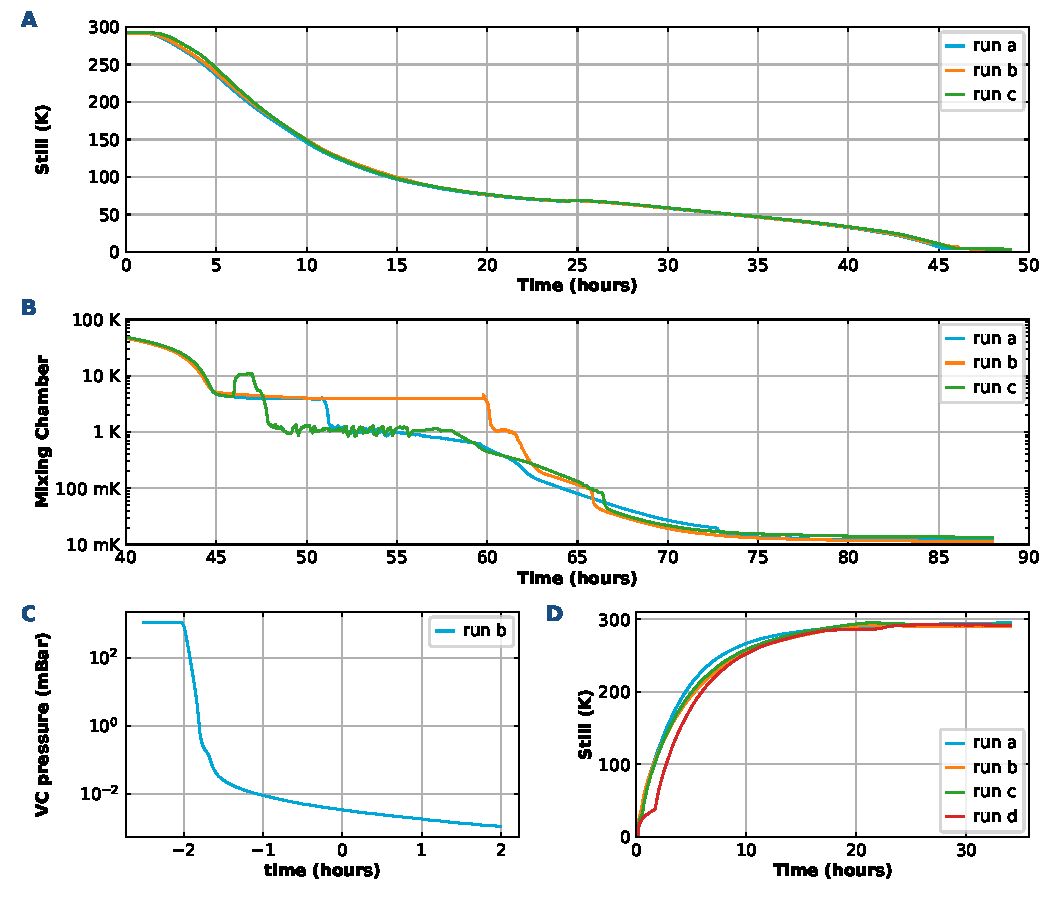
\includegraphics{fig/pagani_performance.pdf}
\caption{\textbf{Pagani Turnaround Performance}
(\textbf{\color{sectioncolor}A}) Initial cooling of the pagani.
(\textbf{\color{sectioncolor}B}) PPC, condensation, and cooling to base temperature.
(\textbf{\color{sectioncolor}C}) Pumping of the VC before cooling.
(\textbf{\color{sectioncolor}D}) Warming up when the run is over.
}
\end{figure}

\begin{figure}[t]
\centering
\textbf{\color{sectioncolor}Lamborghini}
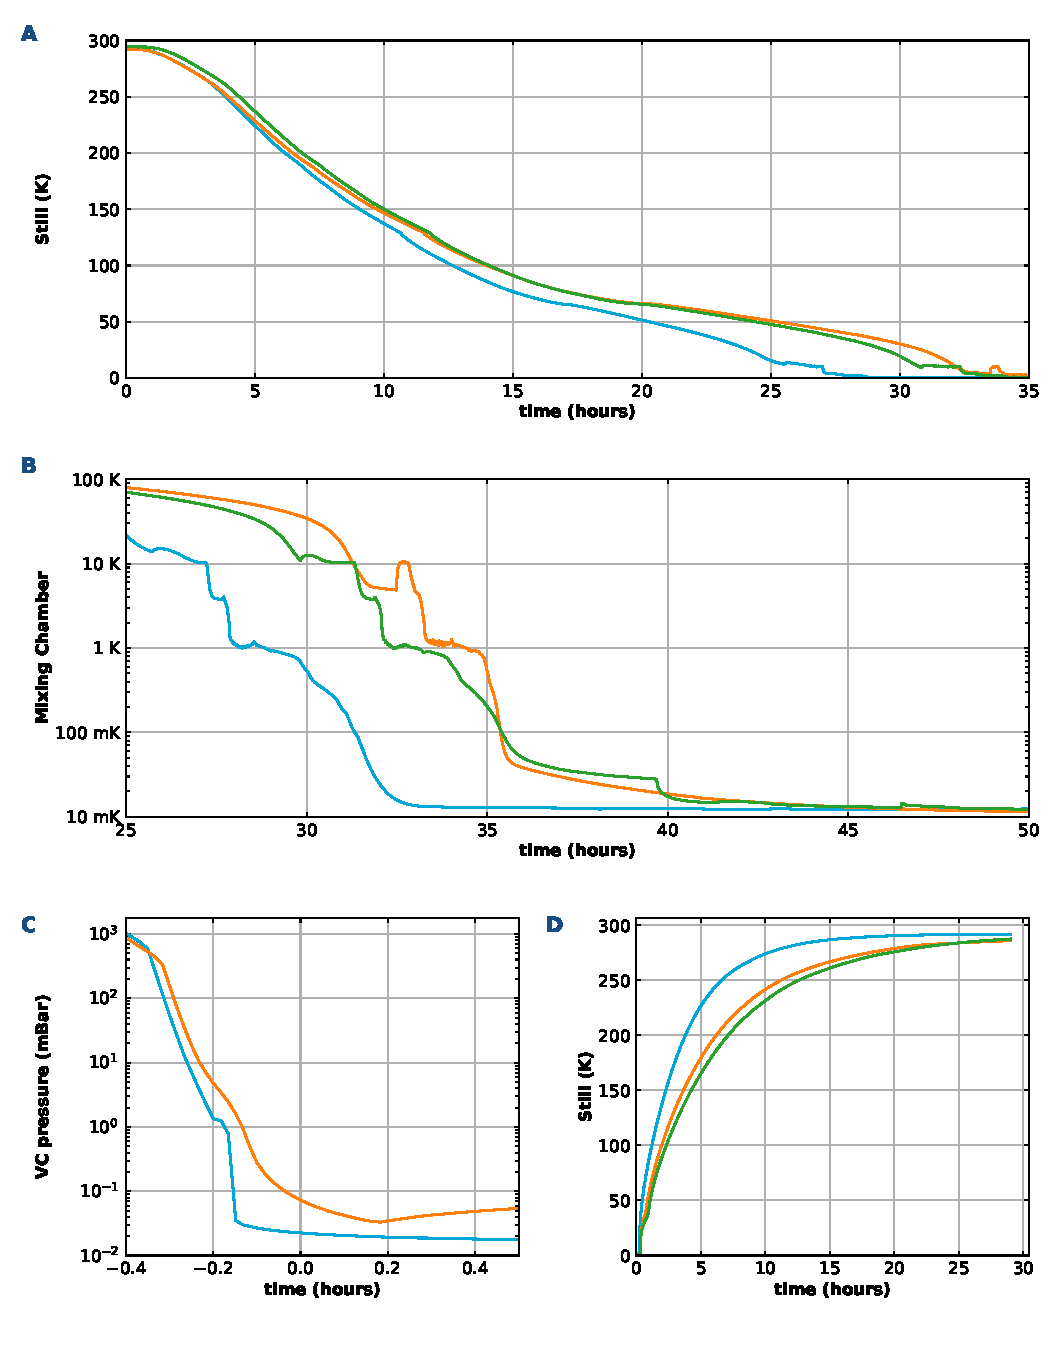
\includegraphics{fig/lamb_performance.pdf}
\caption{\textbf{Lamborghini Turnaround Performance}
(\textbf{\color{sectioncolor}A}) Initial cooling of the Lamborghini.
(\textbf{\color{sectioncolor}B}) PPC, condensation, and cooling to base temperature.
(\textbf{\color{sectioncolor}C}) Pumping of the VC before cooling.
(\textbf{\color{sectioncolor}D}) Warming up when the run is over.
}
\end{figure}






\end{document} 
